\documentclass[12pt]{article}

\usepackage{graphics}
\usepackage{epsfig}
\usepackage{times}
\usepackage{amsmath}
\usepackage{xspace}
\usepackage[nolineno,noindent,norules]{lgrind}
\usepackage{subfig,graphics,graphicx,color}
\DeclareGraphicsExtensions{.eps}

%%\makeatletter
%%\def\v#1{{\mbox{\fontfamily{cmtt}\fontsize{\f@size}{\f@size}\selectfont #1}}}
%%\let\v\texttt
\let\vv\texttt

%% Title stuff.
\newcommand{\mykeywords}[0]{Deterministic Multithreading, Stable 
Multithreading, Reliability, Security, Software Model Checking,
State Space Reduction, State Machine Replication}

\newcommand{\thesistitle}{Stable Multithreading: A New Paradigm for Reliable and Secure Threads}
\newcommand{\thesisauthor}{Heming Cui}
\newcommand{\thesisyear}{2014}

%% Terminology of our own internal techniques.
\newcommand{\compute}{soft barrier\xspace}
\newcommand{\vcompute}{\emph{soft barrier}\xspace}
\newcommand{\computes}{soft barriers\xspace}
\newcommand{\Compute}{Soft barrier\xspace}
\newcommand{\Computes}{Soft barriers\xspace}
\newcommand{\nondet}{performance critical section\xspace}
\newcommand{\vnondet}{\emph{performance critical section}\xspace}
\newcommand{\nondets}{performance critical sections\xspace}
\newcommand{\Nondet}{Performance critical section\xspace}
\newcommand{\Nondets}{Performance critical sections\xspace}

%% Systems and techniques names.
\newcommand{\dmt}[0]{DMT\xspace}
\newcommand{\smt}[0]{StableMT\xspace}
\newcommand{\racepro}[0]{\textsc{RacePro}\xspace}
\newcommand{\tern}[0]{\textsc{Tern}\xspace}
\newcommand{\peregrine}[0]{\textsc{Peregrine}\xspace}
\newcommand{\parrot}[0]{\textsc{Parrot}\xspace}
\newcommand{\msmr}[0]{\textsc{Crane}\xspace}
\newcommand{\grace}[0]{Grace\xspace}
\newcommand{\coredet}[0]{\textsc{CoreDet}\xspace}
\newcommand{\kendo}[0]{Kendo\xspace}
\newcommand{\dthreads}[0]{\textsc{DThreads}\xspace}
\newcommand{\determinator}[0]{Determinator\xspace}
\newcommand{\dbug}[0]{\textsc{dbug}\xspace}
\newcommand{\ecosys}[0]{\parrot-\dbug}
\newcommand{\paxos}[0]{\textsc{Paxos}\xspace}

%% Application names.
\newcommand{\http}{HTTP\xspace}
\newcommand{\apache}{\vv{Apache}\xspace}
\newcommand{\ab}{\vv{ApacheBench}\xspace}
\newcommand{\mysql}{\vv{MySQL}\xspace}
\newcommand{\sysbench}{\vv{SysBench}\xspace}
\newcommand{\mplayer}[0]{{MPlayer}\xspace}
\newcommand{\mencoder}[0]{\vv{mencoder}\xspace}
\newcommand{\pbzip}[0]{\vv{PBZip2}\xspace}
\newcommand{\aget}[0]{\vv{aget}\xspace}
\newcommand{\mongoose}[0]{\vv{Mongoose}\xspace}
\newcommand{\pfscan}[0]{\vv{pfscan}\xspace}
\newcommand{\fft}[0]{\vv{fft}\xspace}
\newcommand{\lu}[0]{\vv{lu}\xspace}
\newcommand{\luc}[0]{\vv{lu\_cb}\xspace}
\newcommand{\lun}[0]{\vv{lu\_ncb}\xspace}
\newcommand{\barnes}[0]{\vv{barnes}\xspace}
\newcommand{\radix}[0]{\vv{radix}\xspace}
\newcommand{\radiosity}[0]{\vv{radiosity}\xspace}
\newcommand{\waters}[0]{\vv{water-spatial}\xspace}
\newcommand{\watern}[0]{\vv{water-nsquared}\xspace}
\newcommand{\oceanncp}[0]{\vv{ocean}\xspace}
\newcommand{\oceancp}[0]{\vv{ocean}\xspace}
\newcommand{\ocean}[0]{\vv{ocean}\xspace}
\newcommand{\fmm}[0]{\vv{fmm}\xspace}
\newcommand{\volrend}[0]{\vv{volrend}\xspace}
\newcommand{\cholesky}[0]{\vv{cholesky}\xspace}
\newcommand{\streamcluster}[0]{\vv{streamcluster}\xspace}
\newcommand{\blackscholes}[0]{\vv{blackscholes}\xspace}
\newcommand{\swaptions}[0]{\vv{swaptions}\xspace}
\newcommand{\bodytrack}[0]{\vv{bodytrack}\xspace}
\newcommand{\bodytrackopenmp}[0]{\vv{bodytrack-openmp}\xspace}
\newcommand{\ferret}[0]{\vv{ferret}\xspace}
\newcommand{\dedup}[0]{\vv{dedup}\xspace}
\newcommand{\raytrace}[0]{\vv{raytrace}\xspace}
\newcommand{\canneal}[0]{\vv{canneal}\xspace}
\newcommand{\racey}[0]{\vv{racey}\xspace}
\newcommand{\freqmine}[0]{\vv{freqmine}\xspace}
\newcommand{\vips}[0]{\vv{vips}\xspace}
\newcommand{\xtwosixfour}[0]{\vv{x264}\xspace}
\newcommand{\fluidanimate}[0]{\vv{fluidanimate}\xspace}
\newcommand{\facesim}[0]{\vv{facesim}\xspace}
\newcommand{\rtviewraytrace}[0]{\vv{rtview\_raytrace}\xspace}
\newcommand{\wordcount}[0]{\vv{word\_count}\xspace}
\newcommand{\klee}[0]{\textsc{klee}\xspace}
\newcommand{\woodpecker}[0]{\textsc{woodpecker}\xspace}
\newcommand{\splashx}[0]{\mbox{SPLASH-2x}\xspace}
\newcommand{\splash}[0]{\mbox{SPLASH-2}\xspace}
\newcommand{\parsec}[0]{\mbox{PARSEC}\xspace}
\newcommand{\phoenix}[0]{\mbox{Phoenix}\xspace}
\newcommand{\pthread}[0]{\mbox{Pthreads}\xspace}

%% Application names (continue).
\newcommand{\kmeans}[0]{\vv{kmeans}\xspace}
\newcommand{\kmeanspthread}[0]{\vv{kmeans-pthread}\xspace}
\newcommand{\linearregre}[0]{\vv{linear-regression}\xspace}
\newcommand{\linearregrepthread}[0]{\vv{linear-regression-pthread}\xspace}
\newcommand{\matrixmult}[0]{\vv{matrix-multiply}\xspace}
\newcommand{\matrixmultpthread}[0]{\vv{matrix-multiply-pthread}\xspace}
\newcommand{\wordcnt}[0]{\vv{word-count}\xspace}
\newcommand{\wordcntpthread}[0]{\vv{word-count-pthread}\xspace}
\newcommand{\stringmatch}[0]{\vv{string-match}\xspace}
\newcommand{\stringmatchpthread}[0]{\vv{string-match-pthread}\xspace}
\newcommand{\histogram}[0]{\vv{histogram}\xspace}
\newcommand{\histogrampthread}[0]{\vv{histogram-pthread}\xspace}
\newcommand{\pca}[0]{\vv{pca}\xspace}
\newcommand{\pcapthread}[0]{\vv{pca-pthread}\xspace}

%% Application names (continue).
\newcommand{\partition}[0]{\mbox{\vv{partition}}\xspace}
\newcommand{\nthelement}[0]{\mbox{\vv{nth\_element}}\xspace}
\newcommand{\partialsort}[0]{\mbox{\vv{partial\_sort}}\xspace}
\newcommand{\ua}[0]{\vv{ua}\xspace}
\newcommand{\is}[0]{\vv{is}\xspace}
\newcommand{\npb}[0]{\mbox{NPB}\xspace}
\newcommand{\imagick}[0]{\mbox{ImageMagick}\xspace}
\newcommand{\openldap}[0]{{OpenLDAP}\xspace}
\newcommand{\redis}[0]{{Redis}\xspace}
\newcommand{\bdb}[0]{{Berkeley DB}\xspace}
\newcommand{\openmp}[0]{{OpenMP}\xspace}
\newcommand{\libgomp}[0]{\vv{libgomp}\xspace}
\newcommand{\vtune}[0]{\vv{VTune}\xspace}

%% imagick programs
\newcommand{\convertshear}[0]{\vv{convert\_shear}\xspace}
\newcommand{\montage}[0]{\vv{montage}\xspace}

\newcommand{\nprog}[0]{108\xspace}
\newcommand{\nrealprog}[0]{55\xspace}
\newcommand{\nstl}[0]{33\xspace}
\newcommand{\nimagick}[0]{14\xspace}
\newcommand{\nparsec}[0]{15\xspace}
\newcommand{\nphoenix}[0]{14\xspace}
\newcommand{\nsplash}[0]{14\xspace}
\newcommand{\nnpb}[0]{10\xspace}
\newcommand{\nbenchmarks}[0]{53\xspace}
\newcommand{\ndatapartition}[0]{86\xspace}
\newcommand{\nprogadhocsync}[0]{5\xspace}
\newcommand{\nprogtimeout}[0]{5\xspace}

\newcommand{\nprognohints}[0]{18\xspace}
\newcommand{\nprogneedhints}[0]{90\xspace}
\newcommand{\nprognondethints}[0]{9\xspace}
\newcommand{\nprognondetandnetwork}[0]{11\xspace} % the UA program is excluded.
\newcommand{\nprognonondethints}[0]{99\xspace}
\newcommand{\nproglineuphints}[0]{81\xspace}
\newcommand{\nproggenericlineuphints}[0]{43\xspace}
\newcommand{\nprogspecificlineuphints}[0]{38\xspace}
\newcommand{\nlineofhints}[0]{109\xspace}
\newcommand{\nlineofcomputehints}[0]{87\xspace}
\newcommand{\nlineofnondethints}[0]{22\xspace}
\newcommand{\hintsperprog}[0]{1.2\xspace}
\newcommand{\nlineupfails}[0]{12\xspace}

%% effects of perfomance hints.
\newcommand{\genericnolineup}[0]{500\%\xspace}
\newcommand{\genericlineup}[0]{0.8\%\xspace}
\newcommand{\specificnolineup}[0]{460\%\xspace}
\newcommand{\specificlineup}[0]{19.1\%\xspace}
\newcommand{\nondetnohints}[0]{830\%\xspace}
\newcommand{\nondethints}[0]{42.1\%\xspace}
\newcommand{\overallnohints}[0]{510\%\xspace}
\newcommand{\overallhints}[0]{11.9\%\xspace}

%% our geometric mean overhead on standard workload.
\newcommand{\meanoverhead}[0]{12.7\%\xspace}
\newcommand{\meanrealoverhead}[0]{6.9\%\xspace}
\newcommand{\meanbenchoverhead}[0]{19.0\%\xspace}

%% model checking reduction.
%% nprogshrink, totally 56: 50 programs with out nondet hints, and 6 programs with network or nondet hints.
\newcommand{\shrinkscale}[0]{$10^{6}$--$10^{19734}$\xspace}
\newcommand{\nprogshrink}[0]{56\xspace}
\newcommand{\nprognondetshrink}[0]{5\xspace}
\newcommand{\nprogverifiedxxx}[0]{99\xspace}
\newcommand{\nprogverifieddbug}[0]{43\xspace}

%% overheads in comparison table.
\newcommand{\nprogcompared}[0]{25\xspace}
\newcommand{\xxxcompoverhead}[0]{11.8\%\xspace}
\newcommand{\dthreadssyncoverhead}[0]{150.0\%\xspace}
\newcommand{\dthreadssyncoverheadnoflui}[0]{112.5\%\xspace}
%\newcommand{\dthreadsoverhead}[0]{1,173\%\xspace}
\newcommand{\dthreadsexampleoverhead}[0]{7.7$\times$\xspace}
\newcommand{\coredetoverhead}[0]{115.1\%\xspace}
\newcommand{\overeach}[0]{10$\times$\xspace}
\newcommand{\overcombined}[0]{4$\times$\xspace}

%% should not use these any more.
\newcommand{\overcoredet}[0]{20.7\xspace}
\newcommand{\overdthreadssync}[0]{131.3\xspace}
\newcommand{\overdthreadsfull}[0]{47.3\xspace}

\newcommand{\npthreadsync}[0]{38\xspace}
\newcommand{\nioync}[0]{33\xspace}
\newcommand{\locsmcmc}[0]{243\xspace}

\newcommand{\eg}{{e.g.}}
\newcommand{\ie}{{i.e.}}
\newcommand{\etc}{{etc}}
\newcommand{\para}[1]{\vspace{.00in}\noindent{\bf #1}}
\newcommand{\wrt}{{w.r.t. }}
\newcommand{\cf}{{cf. }}
\newcommand{\vs}{{vs.}\xspace}

%% Misc.
\newcommand{\github}[0]{\url{github.com/columbia/smt-mc}}
\newcommand{\bug}{\ding{54}\xspace}
\newcommand{\nobug}{\ding{52}\xspace}
\newcommand{\memsched}[0]{\mbox{mem-schedule}\xspace}
\newcommand{\syncsched}[0]{\mbox{sync-schedule}\xspace}
\newcommand{\memscheds}[0]{\mbox{mem-schedules}\xspace}
\newcommand{\acmtechnews}[0]{\vv{ACM TechNews}\xspace}
\newcommand{\tgdaily}[0]{\vv{TG Daily}\xspace}
\newcommand{\physorg}[0]{\vv{Physorg}\xspace}
\newcommand{\syncscheds}[0]{\mbox{sync-schedules}\xspace}

%% Reference stuff.
\usepackage[square,comma,numbers,sort]{natbib}
\usepackage{hypernat}
\usepackage{hyperref}
\hypersetup{
  colorlinks=false,
  pdfborder={0 0 0},
  pdftitle={\mytitle},
  pdfkeywords={\mykeywords},
  bookmarksnumbered,
  pdfstartview={FitH},
  urlcolor=cyan,
  pdfpagelabels=true,
  pdfdisplaydoctitle=true,
}



% <http://psl.cs.columbia.edu/phdczar/proposal.html>:
%
% The standard departmental thesis proposal format is the following:
%        30 pages
%        12 point type
%        1 inch margins all around = 6.5   inch column
%        (Total:  30 * 6.5   = 195 page-inches)
%
% For letter-size paper: 8.5 in x 11 in
% Latex Origin is 1''/1'', so measurements are relative to this.

\topmargin      0.0in
\headheight     0.0in
\headsep        0.0in
\oddsidemargin  0.0in
\evensidemargin 0.0in
\textheight     9.0in
\textwidth      6.5in

\title{
%%{\bf Doctoral Thesis Proposal} \\
\bf \mytitle}
\author{ {Heming Cui}  \\
Department of Computer Science \\
Columbia University\\
{\small heming@cs.columbia.edu}
}
\date{\today}

\begin{document}
\pagestyle{plain}
\pagenumbering{roman}
\maketitle

\pagebreak
\begin{abstract}
Multithreaded programs are notoriously hard to get right, and a key reason is:
these programs have \emph{too many} possible thread interleavings (or
schedules) at runtime. It is extremely challenging for existing techniques to
test, analyze, or verify all these schedules, making multithreaded programs
prone to various reliability and security bugs. This article introduces
 Stable multithreading (\smt), a new idea that can greatly
 reduce the number of possible schedules for multi-threaded programs on all
 inputs with reasonable performance overhead, making
 these programs much easier to get right. This article also presents three
 \smt software systems, \tern, \peregrine, and \parrot, with each addressing
 distinct research challenges. To show that \smt can greatly improve software
 reliability and security, this article describes two promising applications of \smt:
 (1) greatly improving schedule coverage of a popular systematic testing technique
 called model checking, and  (2) enabling transparent state-machine replication for multi-threaded programs.

\end{abstract}

\pagebreak
\tableofcontents
\pagebreak

\cleardoublepage
\pagenumbering{arabic}

\section{Introduction} \label{sec:intro}

Multithreaded programs are difficult to write, test, and debug.  A key
reason is nondeterminism: different runs of a multithreaded
program may show different behaviors, depending on how the threads
interleave~\cite{lee06}.
% We term the interleaved executions of threads a schedule.

Two main factors make threads interleave nondeterministically.  The first
is \emph{scheduling}, how the OS and hardware schedule threads.
Scheduling nondeterminism is not essential and can be eliminated without
affecting correctness for most programs.  The second is \emph{input}, what
data (\emph{input data}) arrives at what time (\emph{input timing}).
% (\eg, when a \v{recv()} call returns).
Input nondeterminism sometimes is essential because major changes in
inputs require different schedules.  However, frequently input
nondeterminism is not essential and the same schedule can be used to
process many different inputs (\S\ref{sec:define-schedule}).  We believe
nonessential nondeterminism should be eliminated in favor of determinism.

% Scheduling nondeterminism is unique to multithreaded programs.  

% Input nondeterminism affects both, but has a unique effect on
% multithreaded programs: make threads interleave differently.  

% for example, pbzip2 
%   compressing and decompressing, 
%   same file blocks

\emph{Deterministic multithreading} (\dmt)
systems~\cite{dmp:asplos09,coredet:asplos10,kendo:asplos09} make threads
more deterministic by eliminating scheduling nondeterminism.
Specifically, they constrain a multithreaded program such that it always
uses the same thread schedule for the same input.  By doing so, these
systems make program behaviors repeatable, increase testing confidence,
and ease bug reproduction.
% \dmt is different from deterministic replay~\cite{r2:osdi, friday2007,
% srinivasan:flashback, revirt, dejavu, vmware-record-replay,
% smp-revirt:vee08, pres:sosp09, scribe:sigmetrics10, odr:sosp09,
% capo:asplos09}, a bug-reproducing technique that often passively records
% execution (\eg, memory accesses/thread schedules) instead of actively
% constraining it.

Unfortunately, though existing \dmt systems eliminate scheduling
nondeterminism, they do not reduce input nondeterminism.  In fact, they
may aggravate the effects of input nondeterminism because of their design
limitation: when scheduling the threads to process an input, they consider
only this input and ignore previous similar inputs.  This stateless design
makes schedules over-dependent on inputs, so that a slight change to
inputs may force a program to (ad)venture into a vastly different,
potentially buggy schedule, defeating many benefits of determinism.  We
call this the \emph{instability} problem. 
This problem is confirmed by our results (\S\ref{sec:bug-stable}) from
an existing \dmt system~\cite{coredet:asplos10}.

In fact, even with the same input, existing \dmt systems may still force a
program into different schedules for minor changes in the execution
environment such as processor type and shared library.  Thus,
developers may no longer be able to reproduce bugs by running their
program on the bug-inducing input, because their machine may differ from
the machine where the bug occurred.

This paper presents \tern, a schedule-centric, stateful \dmt system.  It
addresses the instability problem using an idea called \emph{schedule
  memoization} that memoizes past working schedules and reuses them for
future inputs.  Specifically, \tern maintains a cache of past schedules and
the input constraints required to reuse these schedules.  When an input arrives,
\tern checks the input against the memoized constraints for a compatible
schedule.  If it finds one, it simply runs the program while enforcing
this schedule.  Otherwise, it runs the program to memoize a schedule and
the input constraints of this schedule for future reuse.  By reusing
schedules, \tern avoids potential errors in unknown schedules.  This
advantage is illustrated in Figure~\ref{fig:idea}.

%   \tern thus achieves stability because many programs frequently reuse
%   schedules ().

A real-world analogy to schedule memoization is the natural tendencies in
humans and animals to follow familiar routes to avoid possible hazards
along unknown routes.  Migrant birds, for example, often migrate along
fixed ``flyways.''  We thus name our system after the Arctic Tern, a bird
species that migrates the farthest among all migrants~\cite{artic-tern-wiki}.  

A second advantage of schedule memoization is that it makes schedules
explicit, providing flexibility in deciding when to memoize certain
schedules.  For instance, \tern allows developers to populate a schedule
cache offline, to avoid the overhead of doing so online.  Moreover,
\tern can check for errors (\eg, races) in schedules and memoize only the
correct ones, thus avoiding the buggy schedules and amortizing the
cost of checking for errors.

To make \tern practical, it must handle server programs which frequently
use threads for performance.  These programs present two challenges for
\tern: (1) they often process client inputs (requests) as they arrive, thus
suffering from input timing nondeterminism, which existing \dmt systems do
not handle and (2) they may run continuously, making their schedules
effectively infinite and too specific to reuse.

\tern addresses these challenges using a simple idea called
\emph{windowing}.  Our insight is that server programs tend to return to the
same quiescent states.
% are done processing a batch of inputs.  Based on this insight,
Thus, \tern splits the continuous request stream of a server into
\emph{windows} and lets the server quiesce in between, so that \tern can
memoize and reuse schedules across windows.  Within a window, it admits
requests only at fixed schedule points, reducing timing nondeterminism.

% effectively turns server programs into ``batch programs.''  
% Based on this observation, \tern breaks continuous request streams into
% windows and let the server program quiesces between two windows.
%% Instead of processing the inputs as they arrive, \tern buffers the inputs
%% in a fix-sized window.  When the window is full or no new inputs arrive
%% for a period of time, \tern processes the (possibly partial) window of
%% uncorrelated inputs all together.  \tern waits for the current window to be
%% fully processed before it moves onto the next window to avoid interference
%% between windows.
%% % isolates windows from each other so that they do not interfere.
%% \tern memoizes the aggregate schedule of a window and later uses it on
%% other windows.


%% For server programs which continuously run for long, it is difficult to
%% reuse their schedules because the schedules become too specific to the
%% long runs.  To tackle this challenge, we propose a variant of schedule
%% memoization that splits the continuous execution of a server program into
%% sub-runs, and memoizes and reuses sub-schedules.  Our key observation is
%% that server programs tend to go back to the same quiescent states once
%% they idle, making it possible to reuse sub-schedules from previous
%% sub-runs.




\begin{figure}[t]
\centering
\includegraphics[width=.5\textwidth]{tern/figures/idea.eps}
\caption{\small{\em Advantage of schedule memoization.}  Each solid shape
  represents an input, and each curved line a schedule.  Schedule
  memoization reuses schedules when possible, avoiding bugs in unknown
  schedules and making program behaviors repeatable across similar
  inputs.}
\label{fig:idea}
\end{figure}

We implemented \tern in Linux.  It runs as ``parasitic''
user-space schedulers within the application's address space, overseeing
the decisions of the OS scheduler and synchronization library.  It
memoizes and reuses synchronization orders as schedules to increase
performance and reuse rates. It tracks input constraints using
\klee~\cite{klee:osdi08}, a symbolic execution engine.  Our implementation
is software-only, works with general C/C++ programs using threads, and
requires no kernel modifications and only a few lines of modification to
applications, thus simplifying deployment.

%% % background on nondeterminism
%% Nondeterminism makes multithreaded programs more difficult to test, debug,
%% and maintain than sequential programs~\cite{lee06} because
%% given the same input, these programs may produce different outputs
%% (including error outputs) across different runs.  Two main factors make
%% multithreaded programs nondeterministic:
%% % \emph{input data} (\eg, contents of a received packet),
%% \emph{input timing} (\eg, when a \v{recv()} returns) and \emph{thread
%%   scheduling} (how the OS and hardware interleave threads).  Thread
%% scheduling is a unique factor to multithreaded programs; input timing
%% makes sequential programs nondeterministic as well, but it affects
%% multithreaded programs more because these programs may immediately
%% process inputs as they arrive.

%% Although new programming languages~\cite{shim:sac09,streamit:cc02} and
%% systems for programs with restricted semantics (\eg,
%% Grace~\cite{grace:oopsla09} for programs with \emph{fork-join}
%% parallelism) can eliminate nondeterminism in thread scheduling or the use
%% of threads all together, the majority of parallel programs today (and
%% likely in the near future) are still multithreaded programs that have
%% general semantics and are written in legacy languages (\eg, C and C++).

%% % threads, conventional synchronization (\eg, locks, semaphores,
%% % conditional variables).

%% % and are written in legacy languages such as C and C++.

%% % one way is to use new languages or restrict what programs can do.
%% % for instance, Grace~\cite{grace-oopsla09}, a novel deterministic
%% % execution engine, is not for general multithreaded programs.

%% % definition of \dmt is too narrow.
%% Deterministic multithreading
%% (\dmt)~\cite{dmp:asplos09,coredet:asplos10,kendo:asplos09} reduces nondeterminism
%% in legacy multithreaded programs by making thread scheduling deterministic.
%% Specifically, ignoring input timing, \dmt constrains an program to always use the
%% same thread schedule for the same input, regardless where and when the program
%% runs.  As shown in previous work~\cite{dmp:asplos09,kendo:asplos09,coredet:asplos10}, this determinism makes
%% program behaviors repeatable, increases testing confidence because the schedules
%% tested are the schedules run in the field, and reproduces bugs easily because
%% developers simply run the program on the same inputs.
%% % and reduces the cost of
%% %multithreaded replicas by eliminating the costly communication among replicas.
%% % simplifies debugging because a buggy run in the field can be easily reproduced
%% % by running the program on the same input (without recording the buggy thread
%% % schedule).  
%% Note that \dmt is different from deterministic replay~\cite{r2:osdi, friday2007,
%% srinivasan:flashback, revirt, dejavu, vmware-record-replay, smp-revirt:vee08,
%% pres:sosp09, scribe:sigmetrics10, odr:sosp09, capo:asplos09}, a bug-reproducing technique that often passively
%% records execution (\eg, memory accesses/thread schedules) instead of actively
%% constraining it.

%% This paper focuses on software-based \dmt for legacy programs because
%% hardware-based schemes~\cite{more} require new hardware not available
%% today and language-based schemes~\cite{more} restrict what developers can
%% write and require program rewrites.  

% identification of the instability problem is a contribution.

%% A key problem with existing \dmt systems is that they consider only the
%% current input without previous inputs when deciding the schedule.  This
%% stateless approach makes the choices of schedules oversensitive to input:
%% though the same input is always processed with the same schedule, slightly
%% different inputs may lead to completely different schedules, making
%% program behaviors \emph{unstable}.  This instability may defeat some
%% benefits of determinism because it forces a program to (ad)venture into a
%% previously unseen schedule for each new input.  For instance, it may
%% complicate program understanding and debugging because program behaviors
%% on slightly different input may be much different.  Worse, it may reduce
%% testing confidence because similar inputs may be processed by much
%% different schedules.  Figure~\ref{fig:idea}(a) illustrates this problem.

% unstable also means difficult to understand and debug.

%% A second problem is that existing \dmt systems do not address input timing
%% nondeterminism at all.  They are designed for batch programs that have
%% their inputs statically defined upfront.  This restriction is clearly at
%% odds with server programs such as Apache and MySQL that have inputs
%% continuously and nondeterministically arrive.

%% This paper presents \tern, a stateful \dmt system that makes program
%% executions stable using an idea we call \emph{schedule memoization}.  This
%% idea is based on the insight that a single schedule can often process many
%% \emph{schedule-equivalent} inputs because it only weakly constrains what
%% inputs it can process.  If a schedule is shown to work on an input,
%% \tern memoizes the schedule.
%% %  and the constraints on the input for the schedule to work.  
%% If a (possibly different) schedule-equivalent input arrives later,
%% \tern simply reuses the memoized schedule, instead of wandering into an
%% unknown schedule, as shown in Figure~\ref{fig:idea}(b).  We name our
%% system after a bird specie for its spatial sense to repeat long migration
%% routes.

%% \tern mitigates input timing nondeterminism in server programs using a
%% simple idea we call \emph{windowing}.  It is based on the observation that
%% server programs tend to go back to the same quiescence states once they
%% are done processing a batch of requests.
%% % effectively turns server programs into ``batch programs.''  
%% % Based on this observation, \tern breaks continuous request streams into
%% % windows and let the server program quiesces between two windows.
%% Instead of processing the inputs as they arrive, \tern buffers the inputs
%% in a fix-sized window.  When the window is full or no new inputs arrive
%% for a period of time, \tern processes the (possibly partial) window of
%% uncorrelated inputs all together.  \tern waits for the current window to be
%% fully processed before it moves onto the next window to avoid interference
%% between windows.
%% % isolates windows from each other so that they do not interfere.
%% \tern memoizes the aggregate schedule of a window and later uses it on
%% other windows.
   
%% \begin{figure}
%% \centering
%% \includegraphics[width=0.5\textwidth]{figures/idea.eps}
%% \caption{{\em Schedule memoization illustration}.  Each curved line in the
%%   figures represents a thread schedule.  For similar inputs, existing \dmt
%%   systems may adventure into drastically different, previously unknown
%%   schedules.  In contrast, \tern repeats the same schedules for similar
%%   inputs.}
%% \label{fig:idea}
%% \end{figure}

%% We implement \tern on Linux.  It requires no new hardware (unlike
%% hardware-based \dmt systems~\cite{dmp:asplos09}) and works with legacy
%% programs using C/C++ and threads (unlike language-based
%% approaches~\cite{shim:sac09, streamit:cc02}).  \tern runs as a
%% ``parasitic'' user-space scheduler within the application's address space,
%% overseeing the decisions of the OS scheduler and synchronization library
%% to make them more deterministic and stable.  This architecture requires no
%% modifications to the OS and only a few lines of modifications to the
%% programs, simplifying deployment.

%% % offline and online

We evaluated \tern on a diverse set of 14 programs, including two server
programs Apache~\cite{apache} and MySQL~\cite{mysql}, a parallel
compression utility \pbzip~\cite{pbzip2}, and 11 scientific programs in
\splash~\cite{splash2}.  Our workload included a Columbia CS web trace and
benchmarks used by Apache and MySQL developers.  Our results show that

\begin{enumerate}

\item \tern is easy to use.  For most programs, we modified only a few
  lines to adapt them to \tern.

\item \tern enforces stability across different inputs.  In particular, it
  reused 100 schedules to process 90.3\% of a 4-day Columbia CS web trace.
  Moreover, while an existing \dmt system~\cite{coredet:asplos10} made
  three bugs inconsistently occur or disappear depending on minor input
  changes, \tern always avoided these bugs.

  % MySQL results?
  % We run \tern over two real HTTP request traces and one real SQL query
  % trace, totalling XXX input requests.  \tern can cover these requests
  % using only XX schedules, with the best schedule covering XX requests.
  % We compare \tern to existing \dmt schemes and show that they require XX
  % times more schedule than \tern.

  % read madan's paper on shallow scheduling dependency.  may cite his
  % paper

  % analytical results?

\item \tern has reasonable overhead.  For nine out of fourteen
  evaluated programs, \tern has negligible overhead or improves
  performance; for the other programs, \tern has up to 39.1\%
  overhead.
  %  \tern has bigger overhead when the applications do little computing.

\item \tern makes threads deterministic.  For twelve out of fourteen
  evaluated programs, the schedules \tern memoized can be deterministically
  reused barring the assumption discussed in \S\ref{sec:impl}.

%%   The scheduled \tern memoized 
%%   more deterministic.  Multithreaded executions with \tern can be 7.97
%%   times more deterministic than without, measured in the edit distance
%%   between memory access sequences.  Moreover, we evaluated \tern against
%%   five real concurrency errors frequently studied in previous
%%   work~\cite{avio:asplos06,ctrigger:asplos09,lu:concurrency-bugs,pres:sosp09}.
%%   \tern can deterministically avoid or reproduce the errors in every case.

\end{enumerate}

Our main conceptual contributions are that we identified the instability
problem in existing \dmt systems and proposed two ideas, schedule
memoization and windowing, to mitigate input nondeterminism.  Our
engineering contributions include the \tern system and its evaluation of
real programs.  To the best of our knowledge, \tern is the first stable
\dmt system, the first to mitigate input timing nondeterminism, and the
first shown to work on programs as large, complex, and nondeterministic as
Apache and MySQL.  \tern demonstrates that \dmt has the potential to be
deployed today.

This paper is organized as follows.  We first present a background
(\S\ref{sec:background}) and an overview of \tern (\S\ref{sec:overview}).
We then describe \tern's interface (\S\ref{sec:annotations}), schedule
memoization for batch programs (\S\ref{sec:batch}), and windowing to
extend \tern to server programs (\S\ref{sec:window}).  We then present 
refinements we made to optimize \tern (\S\ref{sec:impl}).  Lastly, we show
our experimental results (\S\ref{sec:evaluation}), discuss related work
(\S\ref{sec:related}), and conclude (\S\ref{sec:conclusion}).

%% Two observations (motivations):

%% First, actually, generating the same input for different exeuctioins are difficult, especially for 
%% interactive applications (e.g., servers and GUI applications).
%% Even input for different executions are the same, the non-deterministic arrival of input will affect executions heavily.  This challenge makes current DMP tools impractical to interactive applications.

%% The second observation is: in many cases, some input does not affect sync order at all. For example, in \pbzip, the contents of the input file does not affect
%% execution, only its size does. This observation inspires us that many input can share the same sync event schedule. However, in these cases, traditional DMP tools which use
%% load/store events to determine sync order may generate totally different sync orders, and this will make their executions overly sensitive to input, which violates their own motivation (deterministic execution) and leads to races.

%% \tern (Execution Carrying Execution), a tool for deterministic multi-threaded executions.

%% Contribution: we are the first work to explore deterministic execution based on input similarity and execution interleaving similarity 
%% (this is an important sentence in the paper, need to digest it again and again).

%% Two main selling points:

%% First, Input similarity. Using sync events and symbolic constraints. Symbolic stable.

%% Second, Execution specification. Use window. Allow software developers to mark start/end of a tasks.
%% Restrict the number of concurrent running tasks.

%% Other selling points: we are at application level, easy to deploy. Anthing else?

%% Our assumption: programs are race free under the given sync-event schedule (weaker than the assumption in Kendo).


\section{Building \smt Systems} \label{sec:done}

Although the vision of stable multithreading is appealing, realizing it
faces numerous challenges.  Three main challenges are:

\begin{enumerate}

\item[$\bullet$] How can we compute the schedules to map inputs to?  The 
schedules
  must be feasible so executions reusing them do not get stuck.
  They should also be highly reusable.

\item[$\bullet$] How can we enforce schedules deterministically and
  efficiently?  ``Deterministically'' so executions that reuse a schedule
  cannot deviate even if there are data races, and ``efficiently'' so
  overhead does not offset reliability benefits.
  This challenge is also a decades-long challenge in the area of
  deterministic execution and replay.

\item[$\bullet$] How can we handle multithreaded server programs?  They often 
run for a
  long time and react to each client request as it arrives, making their
  schedules very specific to a stream of requests and difficult to reuse.

\end{enumerate}

Over the past four years, we have been tackling these challenges and
building \smt systems, which resulted in two \smt prototypes,
\tern~\cite{cui:tern:osdi10} and \peregrine~\cite{peregrine:sosp11}, that
frequently reuse schedules with low overhead.  This section describes our
solutions to these challenges.  Our solutions are by no means the only
ones; subsequent to \tern, others have also built a system that
stabilizes schedules for general multithreaded programs~\cite{dthreads:sosp11}.



\section{\tern: Computing Highly-reusable Schedules} \label{sec:tern}

%% how to collect schedules?
%% from dynamic executions
%% schedule memoization idea and advantages
%%
%% why precondition
%% example of pbzip:
%% results: frequently reuse schedules

Crucial to implementing \smt is how to compute the set of schedules for
processing inputs.  At the bare minimum, a schedule must be feasible when
enforced on an input, so the execution does not get stuck or deviate from
the schedule.  Ideally, the set of schedules should also be small for
reliability.  One possible idea is to pre-compute schedules using static
source code analysis, but the halting problem makes it undecidable to
statically compute schedules guaranteed to work dynamically.  Another
possibility is to compute schedules on the fly while a program is running,
but the computations may be complex and their overhead high.

Instead, we compute schedules by recording them from past executions; the
recorded schedules can then be reused on future inputs to stabilize
program behaviors.  \tern, our system implementing this idea, works as
follows.  At runtime, it maintains a persistent cache of schedules
recorded from past executions.  When an input arrives, \tern searches the
cache for a schedule compatible with the input.  If it finds one, it
simply runs the program while enforcing the schedule.  Otherwise, it runs
the program as is while recording a new schedule from the execution, and
saves the schedule into the cache for future reuse.

The \tern approach to computing schedules has several benefits. First, by
reusing schedules shown to work, \tern may avoid potential errors in
unknown schedules, improving reliability.  A real-world analogy is the
natural tendencies in humans and animals to follow familiar routes to
avoid possible hazards along unknown routes.  Migrant birds, for example,
often migrate along fixed flyways.  Why don't our multithreading systems
learn from them and reuse familiar schedules?  (The name \tern comes from
the Arctic Tern, a bird species that migrates the farthest among all
animals%~\cite{artic-tern-wiki}
.)

Second, \tern explicitly stores schedules, so developers and users can
flexibly choose what schedules to record and when.  For instance,
developers can populate a cache of correct schedules during testing and
then deploy the cache together with their program, improving testing
effectiveness and avoiding the overhead to record schedules on user
machines.  Moreover, they can run their favorite checking tools on the
schedules to detect a variety of errors, and choose to keep only the
correct schedules in the cache.

Lastly, \tern is efficient because it can amortize the cost of computing
schedules.
%recording and checking one schedule over many executions that reuse the
%schedule.
Specifically, recording and checking a schedule is more expensive than
reusing a schedule,
% because \tern has to track more things.  Fortunately, 
but, fortunately, \tern does it only once for each schedule and then
reuses the schedule on many inputs, amortizing the cost.

A key challenge facing \tern is to check that an input is compatible with
a schedule before executing the input under the schedule.  Otherwise, if
\tern tries to enforce a schedule, for instance, of two threads on an input
that requires four, the execution would not follow the schedule.  This
challenge turns out to be the most difficult one we must solve in building
\tern.  Our final solution leverages several advanced program
analysis techniques, including two new ones we
invent.  We refer interested readers to our
papers~\cite{cui:tern:osdi10,peregrine:sosp11} for details, and only
describe the high level idea here.

When recording a schedule, \tern tracks how the synchronizations in the
schedule depend on the input.  It captures these dependencies into 
a relaxed, quickly checkable set of
constraints called the \emph{precondition} of the
schedule.  It then reuses the schedule on all inputs satisfying the 
precondition,
avoiding the runtime cost of recomputing schedules.

A na\"ive way to compute the precondition is to collect constraints from
all input-dependent branches in an execution.  For instance, if a branch
instruction inspects input variable \v{X} and goes down the true branch,
we add a constraint that \v{X} must be nonzero to the precondition.  A
precondition computed this way is sufficient, but it contains many
unnecessary constraints concerning only thread-local computations.  Since
an over-constraining precondition decreases schedule-reuse rates, \tern
removes these unnecessary constraints from the precondition.

\begin{figure}[t]
\centering \tiny \lgrindfile{tern/code/pbzip2.cpp.lineno}
\caption{{\it An example program based on parallel compression utility
  \pbzip.}  It spawns \v{nthread} worker threads, splits a file among the
  threads, and compresses the file blocks in parallel.} \label{fig:pbzip2}
\end{figure}

\begin{figure}[t]
\centering
\begin{minipage}[c]{.9\linewidth}
\tiny \lgrindfile{tern/code/pbzip2-sync-order.cpp}
%\includegraphics[width=.4\textwidth]{figures/pbzip2-sync-order.eps}
\end{minipage}
\caption{{\it A synchronization schedule of the example program.}  Each
  synchronization is labeled with its line number in
  Figure~\ref{fig:pbzip2}.} \label{fig:pbzip2-sync-order}
\end{figure}

\begin{figure}[t]
\centering
\begin{minipage}[c]{0.6\linewidth}
\tiny \lgrindfile{tern/code/pbzip2-constraints.cpp}
\end{minipage}
\caption{{\it All input constraints collected for the schedule.}  Each
  constraint is labeled with its line number in
  Figure~\ref{fig:pbzip2}. Constraints collected from function
  \v{compress} are later removed by \tern because they have no effects on
  the schedule.  The remaining constraints simplify to
  $nthread=2$.} \label{fig:pbzip2-constraints}
\end{figure}

We illustrate how \tern works using a simple program based on the
aforementioned parallel compression utility \pbzip.
Figure~\ref{fig:pbzip2} shows this example. Its input includes all command
line arguments in \v{argv} and the input file data.
To compress a file, it spawns \v{nthread} worker threads,
splits the file accordingly, and compresses the file blocks in parallel by
calling function \v{compress}. To coordinate the worker threads, it uses a
synchronized work list. (Here we use work-list synchronization for
clarity; in practice, \tern handles Pthread synchronizations.) The example
actually has a bug: it is missing \v{pthread\_join} operations at line 7,
so the work list may be used by function \v{worker} after it is cleared at
line 8, causing potential program crashes. This bug is based on a real
bug in \pbzip.

We first illustrate how \tern records a schedule and its precondition.
Suppose we run this example with two threads, and \tern records a schedule
as shown in Figure~\ref{fig:pbzip2-sync-order}, which avoids the
use-after-free bug.  (Other schedules are also possible.)
% To record this schedule, \tern controls and records the synchronizations
% at lines 4, 6, 8, and 11.
To compute the precondition of the schedule, \tern first records the
outcomes of all executed branch statements that depend on input data.
Figure~\ref{fig:pbzip2-constraints} shows the set of constraints
collected.  It then applies advanced program analyses to remove the
constraints that concern only local computations and have no effects on
the schedule, including all constraints collected from function
\v{compress}.  The remaining ones simplify to $nthread=2$, which forms the
precondition of the schedule.  \tern stores the schedule and precondition
into the schedule cache.

We now illustrate how \tern reuses a schedule.  Suppose we want to
compress a completely different file also with two threads.  \tern will
detect that \v{nthread} satisfies $nthread=2$, so it will reuse the
schedule in Figure~\ref{fig:pbzip2-sync-order} to compress the file,
regardless of the file data.  This execution is reliable because the
schedule avoids the use-after-free bug.  It is also efficient because the
schedule orders only synchronizations and allows the \v{compress}
operations to run in parallel.  Suppose we run this program again with
four threads.  \tern will detect that the input does not satisfy the
precondition $nthread=2$, so it will record a new schedule and
precondition.

\subsection{\tern Evaluation} \label{sec:tern-eval}
In this section, we describe the main results of \tern, our first \smt
system.  We focus on two evaluation questions:

\begin{enumerate}

\item[\S\ref{sec:tern-stable}:] Can \tern frequently reuse schedules?  The
  higher the reuse rate is, the more stable program behaviors become, and
  the more efficient \tern is.

\item[\S\ref{sec:tern-efficient}:] Can \tern efficiently enforce schedules?  A
  low overhead is crucial for programs that frequently reuse schedules.

%% \item[\S\ref{sec:deterministic}:] Can \tern deterministically enforce
%%   schedules even if there are data races?  \tern is also deterministic,
%%   so it should preserve the benefits of determinism.

%% \item[\S\ref{sec:precise}:] Can \tern drastically improve the precision
%%   of sound program analysis?  The more precise, the more useful stable
%%   multithreading is at bettering program analysis.

%% \item[\S\ref{sec:annotation}:] Can \xxx significantly reduce manual
%%   annotation overhead?  Recall that our previous
%%   work~\cite{cui:tern:osdi10} required developers to manually annotate the
%%   input affecting schedules.

\end{enumerate}

We choose a diverse set of 14 programs as our evaluation benchmarks.
These programs are either widely used real-world parallel programs, such
as \apache and \pbzip, or parallel
implementations of computation-intensive algorithms in standard benchmark
suites.

\subsubsection{Stability} \label{sec:tern-stable}

\begin{table}[t]
\centering
\small
\begin{tabular}{lcc}
{\bf Program-Workload} & {\bf Reuse Rates (\%)} & {\bf Schedules} \\
\hline
\apache-trace          &   90.3\%    &    100      \\
\mysql-simple          &   94.0\%    &    50      \\
\mysql-tx              &   44.2\%    &    109      \\
\pbzip-usr             &   96.2\%    &    90      \\
\end{tabular}
\vspace{-.05in}
\caption{{\em Schedule reuse rates under four workloads.}  Column {\bf
    Schedules} indicates the number of schedules in the schedule cache.}
\label{tab:stability}
\vspace{-.05in}
\end{table}

We evaluate \tern's stability by measuring the schedule reuse rates under
given workloads.  Table~\ref{tab:stability} shows the results, obtained
from \tern.  The four workloads
are either real workloads collected by us or synthetic workloads used by the
developers themselves~\cite{cui:tern:osdi10}. %(\S\ref{sec:workloads}).
For three out of the four
workloads, \tern reuses a small number of schedules to process over
90\% of the workloads.  For \mysql-tx, \tern has a lower reuse rate
largely because the workload is too random to reuse schedules.
%% Second, we annotated only the SQL command as symbolic
%% without exposing the hidden states of MySQL (\S\ref{sec:window}) so that
%% we could measure \tern's performance in an adversarial setting
Nonetheless, it still processes 44.2\% of the workload.

\begin{figure}[t]
\centering
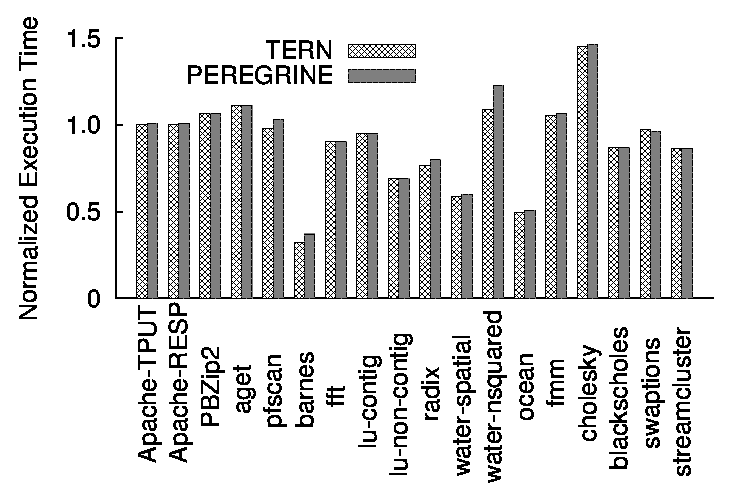
\includegraphics[width=.8\columnwidth]{tern/figures/overhead}
\vspace{-.3in}
\caption{{\em Relative overhead when reusing schedules.} } \label{fig:tern-overhead}
\vspace{-.05in}
\end{figure}


\subsubsection{Efficiency} \label{sec:tern-efficient}

Figure~\ref{fig:overhead} shows the relative overhead of \tern over
nondeterministic execution when reusing schedules, the smaller the better.  For seven out of
the fourteen programs, the replayer performed almost identically to
nondeterministic execution. For \pbzip and barnes, \tern performed
better.  This speedup came partially from the optimization to remove
unnecessary synchronizations~\cite{cui:tern:osdi10}.  \tern's overhead
for MySQL, volrend, raytrace, water-nsquared, and choleskey is relatively
large because these programs performed many synchronization operations
over a short period of time.  For instance, water-nsquared and cholesky
both call \v{pthread\_mutex\_lock()} and \v{pthread\_mutex\_unlock()} in a
tight loop.






\subsection{Peregrine} \label{sec:peregrine}
TBD



\section{Parrot} \label{ch:parrot}


%%\input{eval/eval}

%%\section{Model Checking} \label{sec:mc}
TBD.




\section{Model Checking} \label{sec:mc}
TBD.

\section{Leveraging \smt to Build Transparent Multithreaded State Machine Replication} \label{sec:replication}

TBD.

\section{Related Work} \label{sec:tern-related}

\noindent
{\bf Deterministic Execution} \tern differs from existing \dmt
systems~\cite{dmp:asplos09,coredet:asplos10,kendo:asplos09} by making
threads stable, \ie, repeating familiar behaviors across different inputs.
Another difference is that \tern reduces timing nondeterminism for server
programs through windowing.

% \tern is a software-only approach for multithreaded programs with general
% semantics (\eg, not fork-join~\cite{grace:oopsla09}) and written in legacy
% languages such as C and C++, in contrast to new programming languages
% (\eg~\cite{shim,streamit}), hardware-based approaches~\cite{dmp:asplos09}, and
% systems for programs with restricted semantics~\cite{grace:oopsla09}.

The closest system to \tern in this category is
Kendo~\cite{kendo:asplos09}, a software-only \dmt system that also
enforces synchronization orders instead of memory access orders for
efficiency.  \coredet~\cite{coredet:asplos10} is another software-only \dmt
system that enforces deterministic memory access orders.  Both systems are
based on logical clocks and have been shown to work on scientific
benchmarks, such as \splash.  The authors of \coredet have noted that a small
modification to the original program leads to a much different
\coredet-instrumented program, which the idea of schedule memoization may
address.  \coredet is a software implementation (with extensions) of
DMP~\cite{dmp:asplos09}, a hardware \dmt system .

Grace~\cite{grace:oopsla09} proposes a novel approach to making C and C++
programs with fork-join parallelism behave like sequential programs.  It
runs each thread within a process and commits memory writes atomically and
deterministically.  It detects memory access conflicts efficiently using
hardware page protection.  Grace has been shown to perform and scale well
on Phoenix benchmarks~\cite{phoenix-benchmarks} and a Cilk~\cite{cilk}
benchmark.  Unlike Grace, \tern aims to make general multithreaded
programs, not just fork-join programs, deterministic and stable.

%Several new program languages can make programs
%written in them deterministic.  Although a language-based approach may be
%the ultimate solution to determinism and stability, existing 

\noindent
{\bf Deterministic Replay} Deterministic
replay~\cite{r2:osdi,friday2007,srinivasan:flashback,revirt,dejavu,vmware-record-replay,smp-revirt:vee08,pres:sosp09,scribe:sigmetrics10,odr:sosp09,capo:asplos09}
aims to replay the exact recorded executions, whereas \tern ``replays''
memoized schedules on different inputs.  Some recent deterministic replay
systems include Scribe, which tracks page ownership to enforce
deterministic memory access~\cite{scribe:sigmetrics10}; Capo, which defines
a novel software-hardware interface and a set of abstractions for
efficient replay~\cite{capo:asplos09}; PRES and ODR, which
systematically search for a complete execution based on a partial
one~\cite{pres:sosp09,odr:sosp09}; and SMP-ReVirt, which uses clever page
protection trick for recording the order of conflicting memory
accesses~\cite{smp-revirt:vee08}.

\noindent
{\bf Concurrency Errors} The complexity in developing multithreaded
programs has led to many concurrency errors~\cite{lu:concurrency-bugs}.  A
significant number of them are not data races, but atomicity and order
errors~\cite{lu:concurrency-bugs}, which can be deterministically
reproduced or avoided using only synchronization orders.

Much work exists on concurrency error
detection~\cite{yu:racetrack:sosp,savage:eraser,racerx:sosp03,lu:muvi:sosp,avio:asplos06,conmem:asplos10},
diagnosis~\cite{racefuzzer:pldi08,ctrigger:asplos09,atomfuzzer:fse08}, and
correction~\cite{dimmunix:osdi08,gadara:osdi08}.  \tern aims to make the
executions of multithreaded programs deterministic and stable, and is
complementary to existing work on concurrency errors.  Specifically,
\tern can use existing work to detect and fix the errors in the schedules
it selects.  Moreover, even for programs free of concurrency errors,
\tern still provides value by making their behaviors repeatable.

\noindent {\bf Symbolic Execution} The combination of symbolic and
concrete executions has been a hot research topic.  Researchers have built
scalable and effective symbolic execution systems to detect
errors~\cite{dart:pldi,cute:fse,godefroid:grammar-fuzzing,godefroid:whitebox-fuzzing,klee:osdi08,yang:malicious-disk:oakland06,cadar:exe:ccs06,s2e:hotdep09,taas:socc10},
block malicious inputs~\cite{castro:bouncer}, and preserve privacy in
error reports~\cite{castro:bug-report-privacy}.  Compared to these
systems, \tern applies symbolic execution to a new domain: tracking input
constraints to reuse schedules.


\section{Research Plan} \label{sec:plan}

My collaborators and I have proposed the new idea of \smt (\S\ref{sec:intro}) that can greatly reduce the number of 
possible schedules for all inputs, and we have built three systems, \tern 
(\S\ref{sec:tern}), \peregrine \S\ref{sec:peregrine}, and \parrot 
(\S\ref{sec:parrot}), with each addressing distinct research challenges. We 
have also quantitatively shown that \smt can improve program 
analysis~\cite{wu:pldi12}, verification~\cite{peregrine:sosp11, wu:pldi12}, 
and model checking (\S\ref{sec:mc}). I plan to implement the 
\msmr (\S\ref{sec:rep}) tate-machine replication system as the last piece o my thesis.
Thus, I plan to defend my thesis in Novermber 2014~\cite{dthreads:sosp11}.
  
%%\subsection{Plan for completion of the research}

%%Table \ref{tab:plan} shows my plan for completion of the research.

%%\begin{table}[hc]
%%\begin{small}
%%\begin{center}
%%\begin{tabular}{lll}
%%Timeline & Work & Progress\\
%%\hline
%%          & XXXXXXXXXXXXXXXXXXXXXXXXXXXXXXXXXXXXX & completed\\
%%Nov. xxxx & XXXXXXXXXXXXXXXXXXXXXXXXXXX & ongoing\\
%%Jan. xxxx & Thesis writting & \\
%%Feb. xxxx & Thesis defense & \\
%%\end{tabular}
%%\end{center}
%%\end{small}
%%\caption{Plan for completion of my research}
%%\label{tab:plan}
%%\end{table}



\pagebreak



\begin{footnotesize}
\bibliographystyle{abbrvnat}
\bibliography{bib/biblio}
\end{footnotesize}

\end{document}


